The invariant torus established in Section~\ref{sec:kam} specifies a bounded conservative motion. We now derive the magnetic commands that sustain it in the damped beam and bound the response of all remaining modes. This construction gives an operating envelope for recurrent motion. A physical-energy constraint then extends clearance control to prescribed endpoint manoeuvres.

\subsection{Realizing the learned dynamics through two magnetic ports}
Let $a_j,v_j$ denote the mass-normalized positions and velocities of all $64$ transverse finite-element modes. Their bias-field frequencies are $\omega_j$, and their tip displacement and rotation coefficients are $b_j,t_j$. A transverse tip force $F$ and a transverse field $B_y$ give
\begin{equation}
\begin{aligned}
 \ddot a_j+\alpha\dot a_j+\omega_j^2a_j&=b_jF+t_jU,\\
 U&=E_0(\vartheta-\sin\vartheta)+\mu B_y\cos\vartheta,\\
 \vartheta&=\sum_jt_ja_j .
\end{aligned}
\label{eq:core-two-port}
\end{equation}
These complete modal coefficients define the plant used below; Supplement~\ref{S-sec:full-fe-kam-control} gives its relation to the assembled finite-element matrices.

For the first two modes, write $a_i=S_iX_i$ with the diagonal scales of Section~\ref{sec:derivation}. Because the learned $h$ contains momentum quartics, velocity determines $Y$ through the implicit relation $h_Y(X,Y)=\operatorname{diag}(S_i)^{-1}v_{1:2}/\omega_0$. If $h_{YY}\succ0$, this relation is locally invertible. Differentiating it along $\dot X=\omega_0h_Y$, $\dot Y=-\omega_0h_X$ gives the desired physical acceleration and hence the feedback
\begin{equation}
\begin{aligned}
 a^{\rm des}_{i,tt}&=S_i\omega_0^2(h_{YX}h_Y-h_{YY}h_X)_i,\\
 \begin{pmatrix}F\\U\end{pmatrix}
 &=A_{\rm mag}^{-1}\left(a^{\rm des}_{1:2,tt}+\alpha v_{1:2}
       +\operatorname{diag}(\omega_1^2,\omega_2^2)a_{1:2}\right),\\
 A_{\rm mag}&=\begin{pmatrix}b_1&t_1\\b_2&t_2\end{pmatrix}.
\end{aligned}
\label{eq:core-feedback}
\end{equation}
Substitution into \eqref{eq:core-two-port} enforces the desired acceleration. Differentiating the velocity relation once more and using invertibility of $h_{YY}$ then recovers both canonical equations.

The force and moment in \eqref{eq:core-feedback} are physically realized by the local field $B(r)=(B_0,B_y)+G(r-r_{\rm tip})$, where
\begin{equation}
\begin{aligned}
 B_y&=\frac{U-E_0(\vartheta-\sin\vartheta)}{\mu\cos\vartheta},\\
 G&=\frac F\mu
 \begin{pmatrix}-\sin\vartheta&\cos\vartheta\\
                 \cos\vartheta&\sin\vartheta\end{pmatrix}.
\end{aligned}
\label{eq:core-field}
\end{equation}
For the dipole $m=\mu(\cos\vartheta,\sin\vartheta)$, direct multiplication gives $Gm=(0,F)$ and $\|G\|_2=|F|/\mu$. Symmetry and zero trace of $G$ satisfy the local source-free curl and divergence constraints. The construction requires independent field and gradient authority, observed modal and tip states, and $|\vartheta|<\pi/2$; it does not assume independently actuated mechanical modes.

\begin{theorem}[Full-model realization of the certified torus]
\label{thm:core-lift}
Suppose the learned Hamiltonian has an analytic embedded two-torus with physical angular frequency $\Omega=2\pi\omega_0\varpi$. Assume $h_{YY}\succ0$ on a domain containing this torus with convex $Y$-fibres for each $X$, $A_{\rm mag}$ is invertible and $\alpha>0$. If the lifted motion stays in the domain $|\vartheta|<\pi/2$ of the available commands, feedback \eqref{eq:core-feedback}--\eqref{eq:core-field} gives an embedded invariant two-torus of the complete finite-dimensional plant. For each low-mode orbit on that torus, higher-mode deviations from its unique quasiperiodic response decay exponentially along closed-loop trajectories that remain in the stated command domain.
\end{theorem}
\begin{proof}
The feedback reproduces the low-mode Hamiltonian exactly. Its demands $F,U$ therefore depend only on the torus phase. With Fourier convention $e^{ik\cdot\phi}$, each higher-mode response is
\begin{equation}
 a^*_{j,k}=\frac{b_jF_k+t_jU_k}
 {\omega_j^2-(k\cdot\Omega)^2+i\alpha(k\cdot\Omega)},\qquad j\geq3.
\label{eq:core-lift-response}
\end{equation}
The denominator is nonzero and its inverse is bounded on real frequencies: at zero its real part is positive, and away from zero its imaginary part is nonzero. Analytic forcing thus gives an analytic response on a possibly smaller strip. Positive definiteness on each convex $Y$-fibre makes $Y\mapsto h_Y(X,Y)$ strictly monotone and injective. The physical low-mode coordinates therefore preserve the torus embedding. Differences between high-mode solutions satisfy homogeneous damped oscillator equations and decay exponentially.
\end{proof}

This lift is derived here from the model and the torus supplied by the external KAM theorem. Its physical angular frequency is approximately $(11.41719351,70.24034116)$ rad/s. The positive-measure family remains a statement about the four-dimensional low subsystem. Without sustained input, the physical beam instead converges to its globally asymptotically stable equilibrium (Supplementary Proposition~\ref{S-prop:unified-global-stability}).

For the COMSOL integral fit, interval bounds give $h_{YY}\succeq0.9999999983I$ on the real $0.3$ box and exclude zero from $\det A_{\rm mag}$. The response and startup estimates in Supplement~\ref{S-sec:full-fe-kam-lift} include all $62$ higher modes and the complete nonlinear forcing remainder. Cubic-Hermite spatial bounds yield the whole-centreline and command limits in Table~\ref{tab:core-operation}. With the low state on the exact certified torus and all higher positions and velocities initially zero, the slope remains below $0.155261$ rad. Hence $\cos\vartheta>0.987971$, closing the feedback-domain condition for every phase and all time.

\begin{table}[t]
\centering
\caption{Rigorous bounds for the COMSOL-integral learned model. Startup means zero higher-mode positions and velocities, with the low state on the certified torus.}
\label{tab:core-operation}
\begin{tabular}{lr}
\toprule
Quantity & Upper bound\\
\midrule
Centreline on response graph & $1.922696$ mm\\
Centreline including startup & $1.970263$ mm\\
Transverse field including startup & $0.921665$ mT\\
Gradient norm including startup & $0.02572538$ T/m\\
\bottomrule
\end{tabular}
\end{table}

Figure~\ref{fig:core-kam-control} shows the full-state realization. Over $12$ s, the low-mode state agrees with an independent Hamiltonian integration to within $1.54\times10^{-10}$ in canonical coordinates. Online COMSOL feedback provides a second implementation check: refining its fixed step from $1$ to $0.125$ ms reduces the four-second tip RMSE against the independent full-state solver from $147.852$ to $3.848\,\mu$m. The analytic and interval estimates supply the all-time bounds in Table~\ref{tab:core-operation}; Supplement~\ref{S-sec:full-fe-kam-control} reports the complete refinement study.

\begin{figure*}[t]
\centering
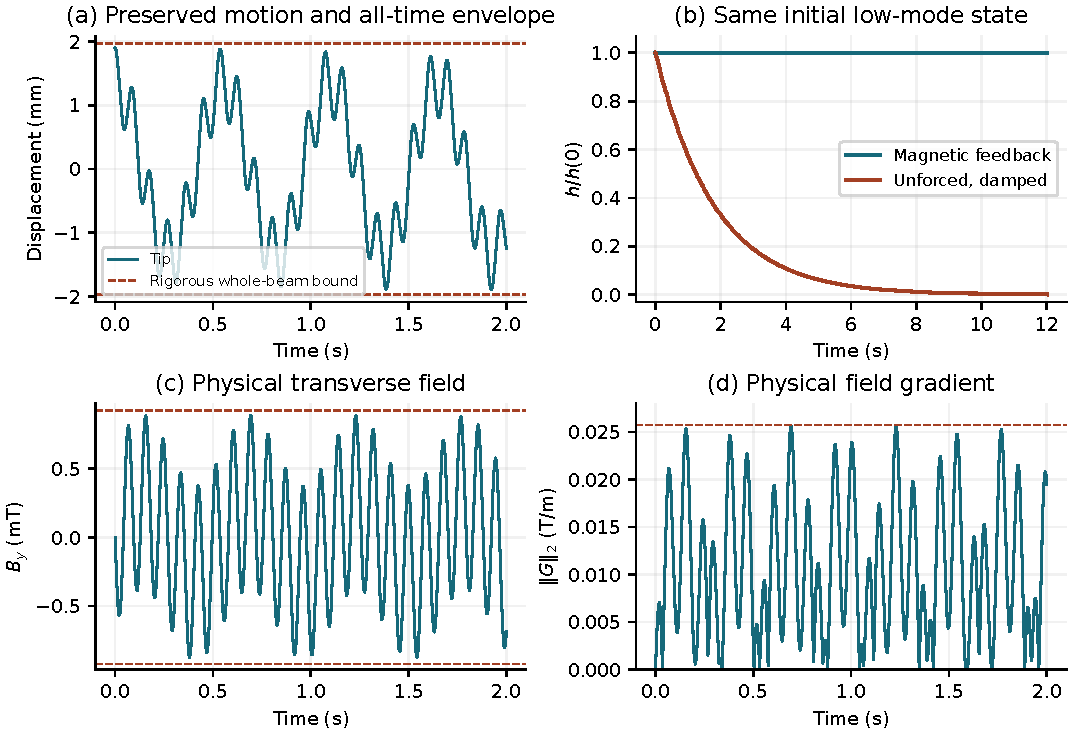
\includegraphics[width=\textwidth]{figures/fig_kam_magnetic_control.pdf}
\caption{Realizing the certified learned dynamics on all $64$ modes. The higher modes start at zero. Dashed envelopes include the startup transient and bound every phase and centreline point. Magnetic field and gradient jointly supply the force and torque; the passive comparison uses the same initial state without this feedback. Panels (a,c,d) show $2$ s and panel (b) shows $12$ s.}
\label{fig:core-kam-control}
\end{figure*}

\subsection{Frequency continuation and the clearance boundary}
To test where driven motion changes character, we vary a single sinusoidal transverse field from $1$ to $20$ mT and its frequency ratio $r=\omega_f/\omega_0$ from $0.7$ to $1.3$. The two-mode physical model is evaluated at $1{,}029$ independently initialized points and $686$ upward/downward continuation points. Each run discards $128$ forcing periods and diagnoses the next $64$ periods. All tested responses converge to forcing-periodic motion; their numerical Floquet spectral radii range from $0.803809$ to $0.889055$. These observations locate no quasiperiodic or chaotic transition within the sampled protocol. Large-deflection extrapolations are separately flagged, and this finite scan does not establish global absence of chaos or breakup of the conservative KAM tori.

A distinct practical boundary appears when periodic bending reaches the $4$ mm clearance. Solving for periodic responses with all $64$ modes gives threshold amplitudes of approximately $7.5005$, $1.91685$ and $8.7909$ mT at $r=0.9$, $1$ and $1.1$, respectively. These are numerical steady-response thresholds; the specified startup ramp can cross the clearance earlier. Supplement~\ref{S-sec:stability-boundary} reports the initial states, continuation protocol, transient thresholds, modal and temporal refinement, and independent full-model checks. The resonance boundary motivates a work constraint that covers transients as well as settled motion.

\subsection{Clearance beyond the invariant torus}
Tracking a prescribed path need not keep the state on a conservative torus. We therefore derive a clearance condition from the physical energy itself. For the clamped small-slope beam, $w(s)=\int_0^s(s-\xi)w_{ss}(\xi)\,d\xi$. Since the static magnetic energy is nonnegative, Cauchy--Schwarz gives
\begin{equation}
 |w(s,t)|^2\leq\frac{2s^3 E(t)}{3EI},\qquad
 E_c=\frac{3EIc^2}{2L^3},
\label{eq:core-clearance}
\end{equation}
where $c$ is the corridor half-width less the rod radius. Thus $E<E_c$ guarantees clearance of the entire centreline and its radius tube. This argument applies to sufficiently regular continuum solutions satisfying the power identity and separately to conforming Hermite finite-element solutions.

For a single transverse magnetic input, its actual power is $a_pB_y$, with $a_p=\mu\cos\vartheta\,\dot\vartheta$. Starting from a valid bound $\overline E_0\geq E(0)$, let $\dot W=a_pB_y$ and $W(0)=\overline E_0$. Nonnegative dissipation gives $E\leq W$. Choose $\overline E_0<E_{\max}<E_c$, and project the requested field onto
\begin{equation}
 |B_y|\leq B_{\max},\qquad
 a_pB_y\leq\kappa(E_{\max}-W),\quad\kappa>0.
\label{eq:core-governor}
\end{equation}
Zero field is feasible while $W\leq E_{\max}$. Moreover, \eqref{eq:core-governor} implies
$E_{\max}-W(t)\geq(E_{\max}-\overline E_0)e^{-\kappa t}$.
Together with \eqref{eq:core-clearance}, this proves all-time clearance under exact port measurement and command application. The result applies to driven trajectories through their supplied work, including motions away from a KAM torus; additional work ports or measurement errors must enter the same budget.

For a $4$ mm net clearance, $E_c=23.8565$ nJ. An energy budget $E_{\max}=0.95E_c$ bounds the centreline by $3.898718$ mm in continuous time. Under a $10$ mT sinusoidal request, the sampled peak falls from $5.14478$ mm without the governor to $3.14362$ mm with it; online COMSOL gives $3.143643$ mm. Supplement~\ref{S-sec:unifiedsafety} supplies the power derivation, an open-loop field-variation bound and refinement data.

\begin{figure*}[t]
\centering
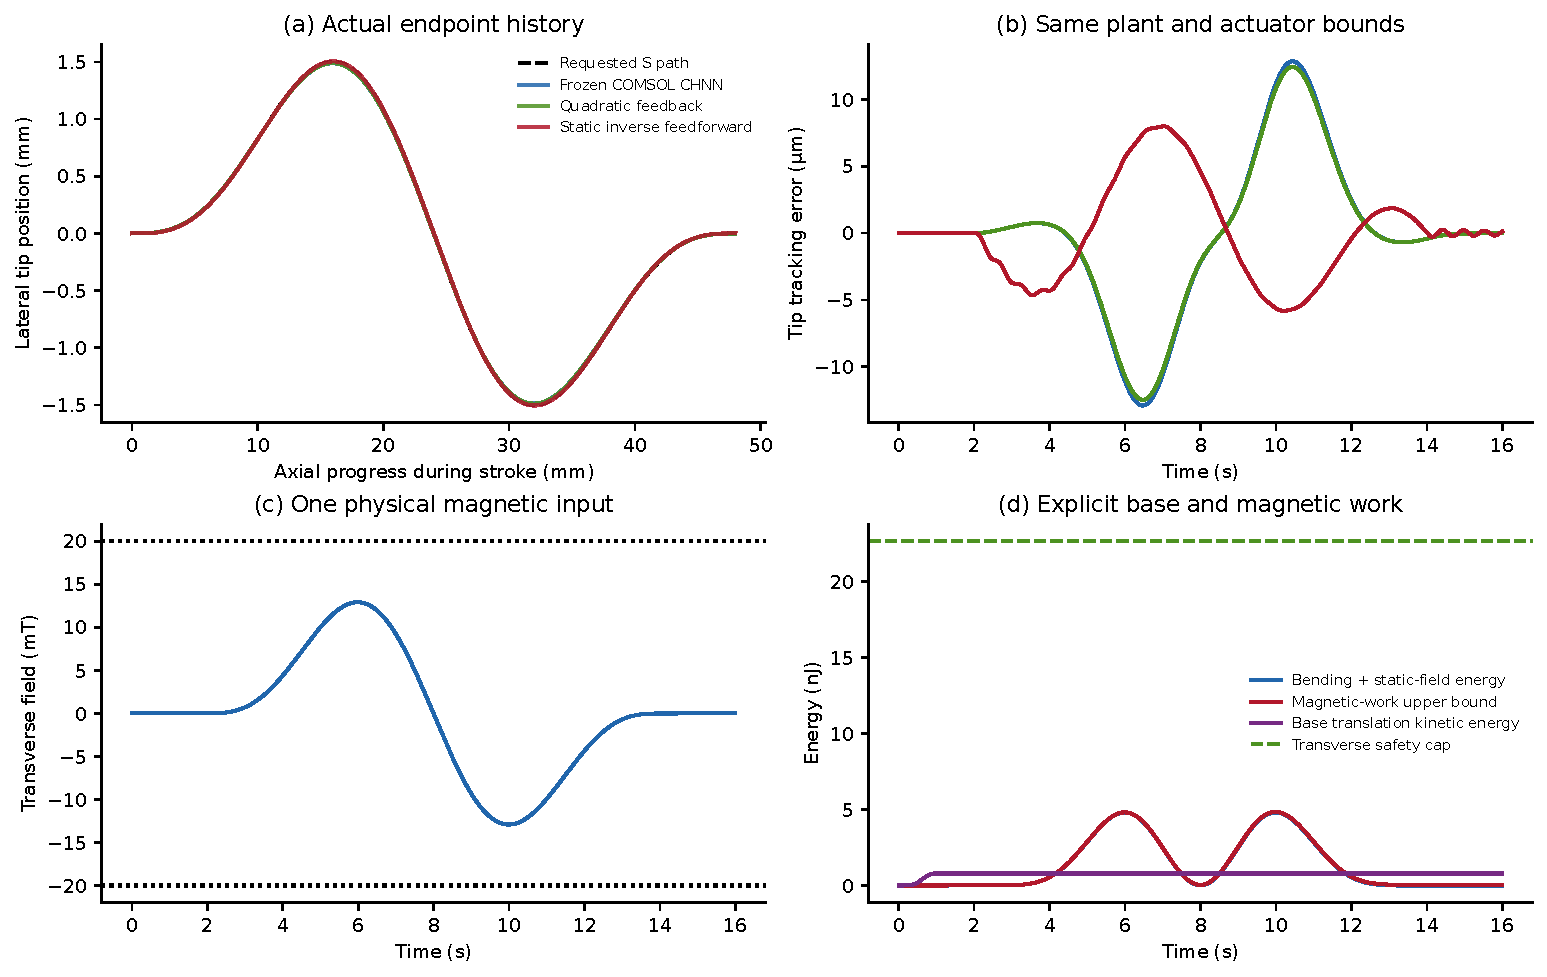
\includegraphics[width=\textwidth]{figures/fig_s_path_tracking.pdf}
\caption{S-shaped endpoint tracking through axial base feed and transverse magnetic actuation. The same full beam and input limits are used for the matched controls. Base work is included in the energy balance.}
\label{fig:core-s-path}
\end{figure*}

\subsection{Nonzero sensing, initialization and actuation tolerances}
The extremely narrow action tube in the KAM measure estimate is a proof domain, rather than an initialization tolerance. A separate physical-energy argument yields a nonzero operating tolerance about the exported finite Fourier reference. In the frozen full nodal model, let $Q(e)=\tfrac12 e_v^{\mathsf T}Me_v+\tfrac12 e_q^{\mathsf T}K_be_q$. The initialization set $Q(e)\leq5$ pJ implies a tip-position error below $56.006\,\mu$m; this is a projection of an energy ellipsoid, not a box of independently admissible coordinate errors.

For the two work ports, bound tip-angle, angular-rate and tip-velocity measurement errors by $1$ mrad, $0.01$ rad/s and $0.1$ mm/s. Allow $1\%$ multiplicative error in both applied inputs, together with additive errors of $0.5$ nN in force and $0.05\,\mu$T in field. A worst-case measured-power bound and a dissipation-based reserve of $0.096780$ nJ cover these additive errors over $4$ s. The resulting $22.66$ nJ energy cap bounds the whole centreline below $3.898405$ mm throughout that interval. Supplement~\ref{S-sec:operational-tolerances} gives the proof, directed-rounding certificate, actuator derating and full-model refinement. The governor can alter the requested motion substantially: this guarantee concerns clearance under the stated errors and does not preserve exact torus membership or certify tracking accuracy.

\subsection{Endpoint tracking and practical scope}
We next combine axial base translation with magnetic bending to trace an S-shaped endpoint path (Figure~\ref{fig:core-s-path}). The tip advances $48$ mm over a $12$ s stroke with lateral extrema $\pm1.5$ mm. Axial acceleration ends before bending begins, and the model has no axial drag or guide contact. With base kinetic energy and work accounted for separately, the transverse governor bounds clearance in the straight corridor (Supplement~\ref{S-sec:s-path}). The prescribed S shape is the moving endpoint trajectory.

The controller uses the two-mode Hamiltonian fitted to full-FE COMSOL trajectories, its full gradient and Hessian, observed low-mode projections and measured tip feedback, with coefficients fixed throughout the task. Table~\ref{tab:core-tracking} compares controllers on the same trajectory and plant with a $20$ mT field limit. The learned controller achieves $6.419\,\mu$m RMS error, while the known-physics inverse performs better on this slow nominal path. The modal-output comparison shows the benefit of using the measured tip in feedback.

\begin{table}[t]
\centering
\caption{Matched S-path controls. RMS errors use the $12$ s stroke; maxima use the complete $16$ s simulation.}
\label{tab:core-tracking}
\setlength{\tabcolsep}{3.5pt}
\begin{tabular}{lrr}
\toprule
Control & RMS ($\mu$m) & Max. ($\mu$m)\\
\midrule
CHNN, tip feedback & 6.419 & 12.907\\
Quadratic, tip feedback & 6.207 & 12.476\\
Static inverse feedforward & 4.124 & 8.005\\
CHNN, modal-output feedback & 25.308 & 41.544\\
\bottomrule
\end{tabular}
\end{table}

The learned command peaks at $12.9177$ mT and the centreline at $1.48892$ mm. The maximum recorded work-based energy estimate is $4.84997$ nJ, and the governor remains inactive for this request. An independent COMSOL replay of the field agrees with the predicted tip to within $4.038\times10^{-10}$ m. The replay tests this task's mechanical response; the torus experiment above additionally tests online feedback.

The resulting design guidance is to preserve fitted energy derivatives, check actuation rank and momentum invertibility, and budget all input work. The envelopes require the stated state estimates and local field/gradient authority. Device implementation requires calibrated hardware and verified error bounds; partial sensing, large rotations, flow and wall contact need corresponding extensions.
